

\documentclass[8pt,final,hyperref={pdfpagelabels=false}]{beamer}
\usepackage{multirow}
\usepackage{hyperref}
\usepackage[orientation=landscape,size=a0,scale=1.4]{beamerposter} % Use the beamerposter package for laying out the poster with a portrait orientation and an a0 paper size
\usepackage{xcolor}
\usetheme{I6pd2} % Use the I6pd2 theme suplied with this template
%\usepackage{extsizes}
\usepackage[english]{babel} % English language/hyphenation

\usepackage{amsmath,amsthm,amssymb,latexsym, subfig}
\usepackage{float}
\usepackage{physics}% For including math equations, theorems, symbols, etc
\theoremstyle{plain}

%\usepackage{times}\usefonttheme{professionalfonts}  % Uncomment to use Times as the main font
%\usefonttheme[onlymath]{serif} % Uncomment to use a Serif font within math environments

\usepackage{booktabs} % Top and bottom rules for tables

\graphicspath{{figures/}} % Location of the graphics files

\usecaptiontemplate{\small\structure{\insertcaptionname~\insertcaptionnumber: }\insertcaption} % A fix for figure numbering
\newcommand\0{\mathbf{0}}
\newcommand\CC{\mathbb{C}}
\newcommand\FF{\mathbb{F}}
\newcommand\NN{\mathbb{N}}
\newcommand\QQ{\mathbb{Q}}
\newcommand\RR{\mathbb{R}}
\newcommand\ZZ{\mathbb{Z}}
\newcommand\bb{\mathbf{b}}
\newcommand\kk{\Bbbk}
\newcommand\mm{\mathfrak{m}}
\newcommand\pp{\mathfrak{p}}
\newcommand\xx{\mathbf{x}}
\newcommand\yy{\mathbf{y}}
\newcommand\GL{\mathit{GL}}
\newcommand\into{\hookrightarrow}
\newcommand\nsub{\trianglelefteq}
\newcommand\onto{\twoheadrightarrow}
\newcommand\minus{\smallsetminus}
\newcommand\goesto{\rightsquigarrow}
\newcommand\nsubneq{\vartriangleleft}
%----------------------------------------------------------------------------------------
%	TITLE SECTION 
%----------------------------------------------------------------------------------------

\title{\huge Theoretical and Performance \\
\vspace{0.8cm}
Comparisons of Single-Mode Codes} % Poster title

\author{Riddhiman Bhattacharya} % Author(s)
\institute{Visvabharati University, Santiniketan, India
}
\newcommand{\leftfoot}{TQC 2024}
\newcommand{\rightfoot}{R. Bhattacharya} 
\begin{document}
\addtobeamertemplate{block end}{}{\vspace*{2ex}}
\begin{frame}
\begin{columns}[t]
\begin{column}{.23\textwidth}                
    \begin{block}{Introduction}
The fundamental objective of quantum error correction entails identifying two logical code words ($\ket{W_\sigma}$), representing a qubit within a vast Hilbert space, that exhibit \textit{robustness} and satisfies Knill-Laflamme Condition: 
$$ \bra{W_\sigma} E_l^\dag E_k \ket{W_\sigma} = \alpha_{l, k} \delta_{\sigma, \sigma'}$$
for all errors $(E_{l,k} \in \mathcal{E})$, where ($\alpha_{l,k}$) denote the elements of a Hermitian matrix that are independent of the logical code words.

      \begin{itemize}
\item non-Hermitian creation/annihilation operators: $a^\dag, a$
\item ${{\begin{aligned}\hat{a}^{\dagger }|n\rangle &={\sqrt {n+1}}|n+1\rangle, \qquad \hat{a}|n\rangle &={\sqrt {n}}|n-1\rangle\end{aligned}}}$
\item $\hat{n} = \hat{a}^{\dag }\hat{a}, \qquad \hat{n}\ket{n} = n\ket{n} $
\item $[\hat{a},\hat{a}^{\dag }]=1,\qquad [\hat{n},\hat{a}^{\dag }]=\hat{a}^{\dag },\qquad [\hat{n},\hat{a}]=-\hat{a},$
\item Coherent states: eigenfunctions of annihilation operator 

$$
|\alpha\rangle =e^{-{|\alpha|^2\over2}}\sum_{n=0}^{\infty}{\alpha^n\over\sqrt{n!}}|n\rangle =e^{-{|\alpha|^2\over2}}e^{\alpha\hat a^\dagger}|0\rangle ~,
$$

\item Note: notation ${\displaystyle |\alpha \rangle }$  does not refer to a Fock/number state.

\item Expression ${\displaystyle |\alpha \rangle } $  with $\alpha = 2$ represents a Poisson distribution of number states ${\displaystyle |n\rangle }$  with a mean photon number of two. 
\item Errors generated by action of $\hat{a}$ :"loss" errors,\\ by $\hat{a}^\dag$ : "gain" errors, and \\ by $\hat{n}$ : "dephasing" errors. 
\end{itemize}
\end{block}
\begin{block}{Single Mode Codes}
\begin{itemize}
\item Simple encoding of $M$ qubits: $2^M$ Fock states cover photon numbers $0, 1, . . . , (2^{M - 1})$.
\item Use binary representation: $\ket{n} = \ket{b_{M-1} b_{M-2} \cdots b_0 }$
\item The $j$th binary digit represents the eigenvalue $(1 + Z_j)/2$ for the corresponding physical qubit. 
\item Photon loss occurs.
\item QEC schemes based on models of independent single qubit errors cannot be easily transferred to this problem.

\end{itemize}
    \end{block}
\begin{block}{Simple Code }
          \begin{itemize}
\item Reminder from quantum optics: mode = frequency + spatial distribution + polarization
\item Protect against $\mathcal{E} = \{ I,a\}$
\item $\ket{W_\uparrow} = \frac{\ket{0} + \ket{4}}{2}$, $\ket{W_\downarrow} = \ket{2}$
\item Hence, $\ket{E_1} = \ket{3}$ and $\ket{E_2} = \ket{1}$



\end{itemize}
\end{block}
\end{column}

\begin{column}{.23\textwidth} % The second column
    
    \begin{block}{Simple Code }
      \begin{itemize}
      \item Distinguish states by measuring number and checking mod 4.
      \item Same mean photon number i.e. $\bra{W_\sigma} n \ket{W_\sigma} = 2$
\begin{itemize}
\item So, $a : \alpha\ket{W_\uparrow} + \beta\ket{W_\downarrow} \mapsto \alpha \ket{E_1} + \beta \ket{E_2}$ (no deformation)
\end{itemize}
\item Generalize
\begin{itemize}
\item Greater spacing between states: can detect higher order loss errors or alternatively gain errors
\item Action by $n$ "dephases". This leads to a superposition of codewords and error words. Project onto word basis to recover (efficient).
\end{itemize}
\end{itemize}
    \end{block} 
    
    \begin{block}{Cat Codes}
\begin{itemize}
\item Superposition of '\textcolor{brown}{well-separated coherent}' states ("legs")
\item $2(L+1)$ legs protects $L$ photon losses. Compare to binomial code with $S=L$
\item E.g. $L=1$

$$
\ket{C^\alpha_{\uparrow/\downarrow}} = \ket{\alpha} \pm \ket{i \alpha} + \ket{-\alpha} \pm \ket{-i \alpha} 
$$

up to a normalization factor.
\item As $\alpha \rightarrow \infty$, $\bra{C^\alpha_{\uparrow}} N^p \ket{C^\alpha_{\uparrow}} = \bra{C^\alpha_{\downarrow}} N^p \ket{C^\alpha_{\downarrow}}$ so potentially immune from unlimited order dephasing.
\item Fock states are distributed as Poisson and for large $N$, Binomial and Poisson approach normal distribution

\end{itemize}
    \end{block}
    
    \begin{block}{Binomial Codes}
\begin{itemize}
\normalsize
\item Protect against $\mathcal{E} = \{I, a, a^2, \cdots, a^L, a^\dag, \cdots, (a^\dag)^G, N, \cdots, N^D \}$
\item Consider

$$
\ket{W_{\uparrow / \downarrow}} = \frac{1}{\sqrt{2^N}} \sum_{ p\text{ even/odd}}^{[0, N+1]} \sqrt{\binom{N+1}{ p }} \ket{p(S+1)}
$$

with $S = L+G$, $N = \max\{L, G, 2D\}$.
\item Mean photon numbers equal (no deformation) and QEC condition holds
\item Can be shown by writing difference in $l^\text{th}$ moment of photon number of codewords as $l^\text{th}$ derivative of $(1+x)^{N+1}\vert_{x=-1}$ with $l \leq \max\{L, G\}$ up to a factor
\item Measure photon number mod $S+1$
\end{itemize}
    \end{block}
\end{column}
\begin{column}{.23\textwidth} % The Third column
        \begin{block}{GKP Codes}
        \begin{itemize}
            \item Constructed based on the continuous basis of non-normalizable eigenstates of the position operator $\hat{x}$. Ideal GKP encompasses both infinite mean photon number and infinite number of states that are perfectly squeezed within the $\hat{x}$ lattice.
            \item Ideal qubit GKP states can be expressed $$\ket{GKP_{\uparrow/\downarrow}} \sim \sum_{p\text{ even/odd}}^{(-\infty, \infty)} \hat{D}\Big(p \sqrt{\frac{\pi}{2}} \Big) \ket{\hat{x} = 0}$$ 	

where,  $\hat{D}(\alpha) = \exp(\alpha \hat{a}^\dag - \alpha^* \hat{a})$
            \item Correctable Errors themselves form a continuous set. 
            \item Protection against displacement error ($\hat{D}(\alpha)$).
            \item The GKP code achieves approximate error correction through the utilization of ancillae states prepared in an equal superposition of logical basis states, homodyne measurements, and incoherent $\chi^{(2)}$ interactions.
        \end{itemize}
    \end{block}
    \begin{block}{Theoretical Comparisons}
        \begin{figure}
            
            \begin{minipage}{0.49\textwidth}
                \centering
                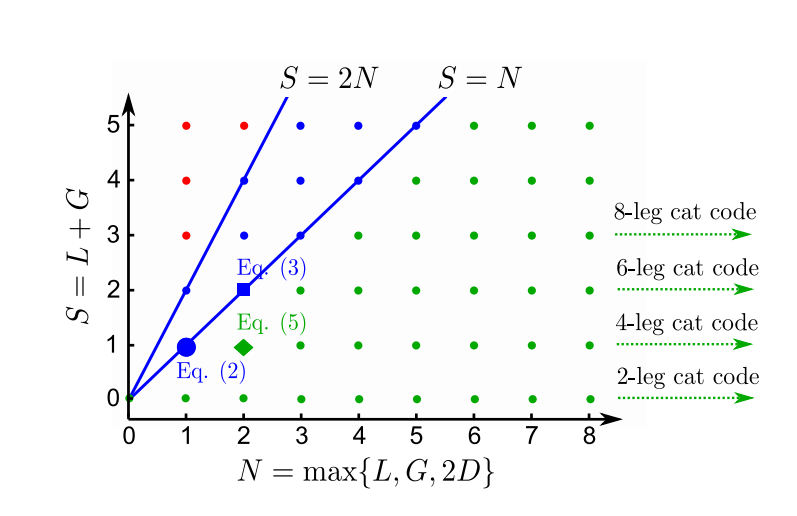
\includegraphics[width=1\linewidth,keepaspectratio]{Screenshot (958).png}	
\caption{Figure comparing binomial codes to cat codes.\cite{michael2016new} }
            \end{minipage}
        \end{figure}
        \begin{itemize}
        \item When considering the average photon number [$\bar n$] for single-loss correction, we find binomial codes outperform cat codes, followed by GKP codes. \\
        $$\text{binomial} > \text{cat} > \text{GKP}$$
        This sequence was deduced by examining the photon number pump needed to satisfy the approximate quantum error correct conditions upto $\kappa\delta t$ order.

            \item Single mode binomial codes and GKP codes necessitate explicit correction gates at each time step, irrespective of whether a photon jump has occurred. 

            
            \item Binomial codes operate within a constant Hilbert space which is advantageous when dealing with errors involving $\hat{a}^\dag$ operators for error detection.
            \item The fock- -state distributions of binomial and cat codes are binomial and Poissonian respectively. So, as the average Photon count increases [larger N],  Binomial and cat codes converges to normal distribution.

        \end{itemize}
    \end{block}
\end{column} 
\begin{column}{.23\textwidth} 
    \begin{block}{Performance Comparisons}

      \begin{itemize}
          \item Channel Fidelity ($F_\varepsilon$) is a feasible measure to assess the efficacy of single-mode bosonic code protection.
          \item If we assume that our noise is entirely characterized by the lossy bosonic channel, the $F_\varepsilon$ measures the degree of overlap between the initial state and final state in the presence of noisy bosonic channel.
          \item  Numerical findings demonstrate codes designed to effectively counter predominant errors at low loss rate ($\gamma$ ) might not necessarily translate into equally effective performance at higher ($\gamma$) values.  \begin{figure}
            
            \begin{minipage}{0.49\textwidth}
                \centering
                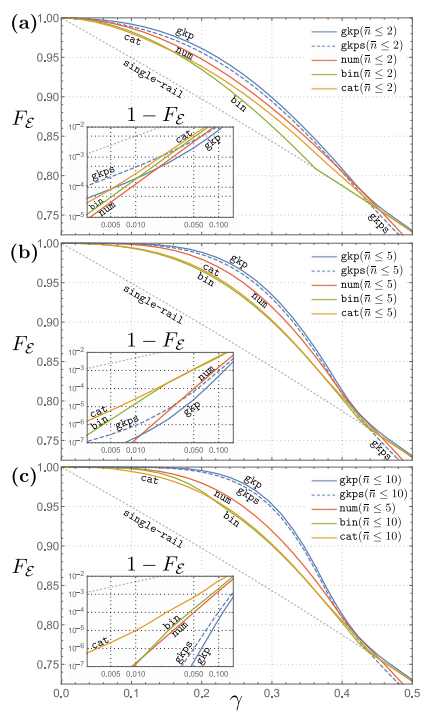
\includegraphics[width=1\linewidth,keepaspectratio]{Screenshot (960).png}	
\caption{Performance evaluation of the optimal code under the constraint of mean photon number, while varying  $\gamma$ }
            \end{minipage}
        \end{figure}
        \item GKP codes achieve the quantum capacity of Gaussian loss channels upto a constant gap relative to an upper bound of the quantum capacity.
        
      \end{itemize}
    
    \end{block}
    \begin{block}{Reference}
        The poster is based on the paper '\href{https://vixra.org/abs/2404.0090}{A Comprehensive Review of Bosonic Quantum Error Correcting Codes}' by
Riddhiman Bhattacharya. 
        \nocite{*} % Include all references from the .bib file
    \bibliographystyle{plain} % Choose a bibliography style
    \bibliography{sample}
    \end{block}

\end{column} 
\end{columns}
\end{frame}

\end{document}